\section{Konstrukcja kraty wykładniczej}

W tym podrozdziale omówię część pracy \cite{10.1145/1007352.1007400}.
Tematem pracy są konstrukcje algorytmów dla problemów K-means oraz K-median.
W kontekście problemu K-means autorzy zaproponowali algorytm bazujący na budowaniu coresetu, który uzyskuje lepszą złożoność od \cite{Matousek99onapproximate}.
Schemat konstrukcji jest następujący:
\begin{itemize}
    \item Obliczmy szybką ale niedokładną aproksymację dla problemu K-means z dużym $k$.
    \item Obliczoną aproksymację przekształcamy w $(\epsilon, k)$ coreset używając kraty wykładniczej.
\end{itemize}


\subsection{Szybka aproksymacja dla problemu K-means.}
\noindent
Zacznijmy od pierwszej części.
Dokładniej udowodnię następujące twierdzenie dla konstrukcji którą opiszę.

\begin{thm}
    Dla danego zbioru $n$ punktów $X \subset \mathbb{R}^d$ oraz parametru $k \in \mathbb{N}^{+}$ możemy 
    obliczyć zbiór $P$ o mocy $O(k \log^{3}n)$ dla którego 
    \begin{equation}
        \phi_{X}(P) \leq 32 \phi_{opt}^{k}(X)
    \end{equation}
    Czas działania algorytmu to $O(n)$ dla $k = O(n^{\frac{1}{4}})$ oraz $O(n \log (k \log n))$ w przeciwnym przypadku.
\end{thm}

% TODO -> rename var

\noindent
Niech $P \in \mathbb{R}^{d}$ to dany na wejściu zbiór $k$ punktów.
Będziemy chcieli szybko obliczyć aproksymację dla problemu K-means na tym zbiorze, gdzie $k$ będzie rzędu $O(k \log^{3}n)$.

\begin{definition}
    \emph{Złe/dobre punkty.} Dla zbioru punktów $X$, punkt $p \in P$ nazywamy \textit{złym} jeżeli
    \begin{equation}
        d(p, X) \geq 2d(p, C_{opt})
    \end{equation}
    gdzie $C_{opt}$ to zbiór punktór realizujący $\phi_{opt}^{k}(P)$.
    Punkt jest \textit{dobry} jeżeli nie jest zły.
\end{definition}

\noindent
Na początku opiszę procedurę która dla danego $P$, wyznacza zbiór centrów $X$ oraz zbiór $P^{'} \subset P$.
Zbiór $P^{'}$ będzie zwierać \textit{dobre} punkty dla zbioru $X$.
\\~\\
Konstrukcję zbioru $X$ zaczynamy od obliczenia 2-aproksymacji problemu k-centrów dla zbioru $P$.
Niech obliczony zbiór centrów to $V$.
Taką aproksymację dla $k = O(n^{\frac{1}{4}})$ możemy obliczyć w czasie $O(n)$ oraz dla $k = \Omega(n^{\frac{1}{4}})$ w czasie $O(n \log k)$ \cite{10.1145/62212.62255}.
Niech $L$ będzie promieniem takiej aproksymacji, czyli największą odległością pomiędzy centrem a punktem $p \in P-V$.
Ponieważ \cite{10.1145/62212.62255} bazuje na \cite{Gonzalez1985ClusteringTM} to dystans pomiędzy dowolną parą punktów z $V$ to conajmniej $L$.
To implikuje następujące ograniczenia:
\begin{equation}
    \Big( \frac{L}{2 } \Big)^2 \leq \phi_{opt}^{k}(V) \leq \phi_{opt}^{k}(P) \leq nL^{2}
\end{equation} 
\\~\\
Następnym krokiem będzie wylosowanie $\rho = \gamma k \log^{2} n$ punktów ze zbioru $P$.
Niech wylosowane punkty to $Y$ oraz $\gamma$ to stała, która wynika z analizy, którą zaraz przeprowadzimy.
Finalnie, $X = Y \cup V$ będzie zbiorem centrów klastów.
Dla $\rho > n$ przyjmujemy $X = P$.
\\~\\
Konstrukcja zbioru $X$ jest stosunkowo prosta.
Dużo cięższym zadaniem jest zbudowanie zbioru $P^{'}$, który jest zbiorem \textit{dobrych} punktów dla $X$.

\subsection{Konstrukcja zbioru dobrych punktów dla $X$.}

Rozpatrzmy zbiór $C_{opt}$, który jest optymalnym zbiorem centrów dla problemu K-means w kontekście $P$.
Dla każdego $c_{i} \in C_{opt}$ tworzymy kulę $b_{i}$ o środku w $c_{i}$.
Każda taka kula będzie zawierać $\eta = \frac{n}{20kk \log n}$ punktów z $P$.
Jeżeli $\gamma$ jest odpowiednio duże to z wysokim prawdopodobieństwem w każdym $b_{i}$ jest przynajmniej jeden punkt z $X$.
Dokładniej:
\begin{equation}
    X \cap b_{i} \neq \emptyset \text{ dla } i = 1 \dots k
\end{equation}

\noindent
Niech $P_{bad}$ będzie zbiorem złych punktów $P$ w kontekście zbioru $X$.
Załóżmy, że dla każdego $b_{i}$ istnieje punkt $x_{j} \in X$, który $x_{j} \in b_{i}$.
Zauważmy, że dla każdego punktu $p \in P \setminus b_{i}$ dla którego $x_{j}$ jest centerm mamy $||px_{j}|| \leq ||pc_{i}||$.
W szczególności takie punkty są \textit{dobre}, dla $c_{i}$ będącymi optymalnymi centrami dla tych punktów.
Zatem z wysokim prawdopodobieństwem jedyne \textit{złe} punkty będą w kulach $b_{i}$ dla $ i = 1, \dots, k$.
To implikuje, że z wysokim prawdopodobieństwem liczba złych punktów w $P$ dla zbioru $X$ to co najwyżej $\beta = k\eta = \frac{n}{20 \log n}$.
\\~\\
W takim razie złych punktów nie jest dużo.
Mimo tego bezpośrednie wyznaczenie tych punktów jest skomplikowane.
Autorzy pracy \cite{10.1145/1007352.1007400} budują zbiór $P^{'}$ tak aby koszt złych punktów w $P^{'}$ był jak najmniejszy.
Koszt w tym kontekście oznacza to jaki wkład ma punkt w wartość $\phi_{P^{'}}(X)$.
Dla każdego punktu w $P$ obliczamy najbliższego sąsiada w $X$.
Niech $r(p) = d(p, X)$ dla każdego punktu $p \in P$.
Teraz podzielimy P na zbiory według następującej formuły:
\begin{equation}
    P[a,b] = \{ p \in P \text{ | } a \leq r(p) \leq b \}
\end{equation}
A dokładniej
\begin{equation}
    P_{0} = P\Big[0, \frac{L}{4n}\Big]
\end{equation}
\begin{equation}
    P_{ \infty } = P\Big[2Ln, \infty \Big]
\end{equation}
\begin{equation}
    P_{i} = P\Big[ \frac{2^{i-1}L}{n}, \frac{2^{i}L}{n} \Big]
\end{equation}
\\~\\
dla $i = 1, \dots, M$, gdzie $M = 2 \lceil \lg n \rceil + 3$.
Taki podział możemy wykonać w czasie linowym.
Niech $P_{\alpha}$ będzię ostatnim zbiorem, który zawiera więcej niż $2\beta = \frac{n}{10 \log n}$. 
Szukany zbiór zdefiniujemy następująco:
\begin{equation}
    P^{'} = V \cup \bigcup_{i \leq \alpha} P_{i}
\end{equation}
gdzie $|P^{'}| \geq \frac{n}{2}$ oraz $\phi_{P^{'}}(X) = O(\phi_{P^{'}}(C_{opt}))$.
Teraz udowodnimy, że faktycznie tak zdefiniowane $P^{'}$ spełnia powyższe założenia.

\begin{proof}
    Moc zbioru $P^{'}$ jest na pewno równa conajmniej $\Big(n - |P_{\infty}| - M\frac{n}{10 \log n} \Big)$.
    Zauważmy, że $P_{\infty} \subseteq P_{bad}$ oraz $|P_{bad}| \leq \beta$.
    A więc:
    \begin{equation}
        |P^{'}| \geq n - \frac{n}{20 \log n} - M \frac{n}{10 \log n}
    \end{equation}
    \begin{equation}
        = n - \Big(\frac{n}{10 \log n}\Big) \Big(M + \frac{1}{2}\Big)
    \end{equation}
    \begin{equation}
        = n - \Big(\frac{n}{10 \log n}\Big) \Big(2 \lceil \lg n \rceil + 3 + \frac{1}{2}\Big)
    \end{equation}
    \begin{equation}
        \geq \frac{n}{2}
    \end{equation}
    Jeżeli $\alpha > 0$ to $|P_{\alpha}| \geq 2\beta = \frac{n}{10 \log n}$.
    Teraz chcemy oszacować jaką kontrybucję w $P^{'}$ mają złe punkty.
    Z uwagi na to jak budujemy $P^{'}$ w najgorszym przypadku wszystkie złe punkty będą w $P_{\alpha}$.
    Wtedy takie punkty będą miały największy wpływ na funkcję $\phi$.
    Niech $Q^{'} = P_{\alpha} \setminus P_{bad}$.
    Dla dowolnego punktu z $p \in P^{'} \cap P_{bad}$ oraz $q \in Q^{'}$, mamy $d(p, X) \leq 2d(q,X)$.
    Dodatkowo $|Q^{'}| > |P_{bad}|$, a więc:
    \begin{equation}
        \phi_{P^{'} \cap P_{bad}}(X) \leq 4\phi_{Q^{'}}(X) \leq 16\phi_{Q^{'}}(C_{opt}) \leq 16\phi_{P^{'}}(C_{opt})
    \end{equation}
    Teraz możemy wyprowadzić następujące ograniczenie:
    \begin{equation}
        \phi_{P^{'}}(X) = \phi_{P^{'} \cap P_{bad}}(X) + \phi_{P^{'} \setminus P_{bad}}(X)
    \end{equation}
    \begin{equation}
        \leq 16\phi_{P^{'}}(C_{opt}) + 4\phi_{P^{'}}(C_{opt}) = 20\phi_{P^{'}}(C_{opt})
    \end{equation}
    Jeżeli $\alpha = 0$ to dla dowolnego punktu $p \in P^{'}$ mamy:
    \begin{equation}
        (d(p,X))^2 \leq n\Big(\frac{L}{4n}\Big)^2 \leq \frac{L^{2}}{4n}
    \end{equation}
    Zatem:
    \begin{equation}
        \phi_{P^{'}}(X) \leq \frac{L^{2}}{4} \leq \phi_{V}(C_{opt}) \leq \phi_{P^{'}}(C_{opt})
    \end{equation}
    gdzie $V \subseteq P^{'}$.
\end{proof}

\noindent
Powyższa analiza dowodzi poprawności konstrukcji dla zbiorów $X$ i $P^{'}$.
Podsumowując otrzymujemy zbiór $X$ o mocy $O(k \log^{2} n)$ oraz zbiór $P^{'}$ dla którego mamy $\phi_{P^{'}}(X) \leq 32\phi_{P^{'}}(C_{opt})$.
Czas działania tego algorytmu to $O(n)$ dla $k = O(n^{\frac{1}{4}})$ oraz $O(n \log (k \log n))$ w przeciwnym przypadku.
Aby otrzymać taką złożoność kluczowe jest szybkie oblicznie najbliższych sąsiadów.
Autorzy proponują \cite{10.1145/293347.293348}.
\\~\\
Wróćmy teraz do twierdzenia 4.1, które zostało zdefiniowane na początku podrozdziału 4.2.
Powyżej zdefiniowaną procedurę powtarzamy dla zbioru $P_{1} = P \setminus P^{'}$.
Analogicznie otrzymamy zbiór $P_{1}^{'}$ oraz $X_{1}$.
Kolejny raz aplikujemy procedurę na zbiorze $P_{2} = P \setminus (P^{'} \cup P_{1}^{'})$.
Ponieważ za każdym razem zbiór $P_{i}$ zmieniejsza się o połowę to taki proces zakończy się po $O(\log n)$ powtórzeniach.
Finalnie otrzymamy zbiór $X \cup X_{1} \dots X_{i}$ o mocy $O(k \log^{3} n)$ dla którego $\phi_{P}(X) \leq 32\phi_{P}(C_{opt})$.
Złożoność pozostanie taka sama, czyli $O(n)$ dla $k = O(n^{\frac{1}{4}})$ oraz $O(n \log (k \log n))$ w przeciwnym przypadku.

\subsection{Krata wykładnicza.}

Przejdzmy teraz do kluczowej części tego podrozdziału, czyli konstrukcji kraty wykładniczej.
Niech $P \subset \mathbb{R}^d$, $|P| = n$ oraz niech $A = \{x_{1}, \dots, x_{m}\}$ będzie zbiorem punktów dla którego zachodzi $\phi_{P}(A) \leq c\phi_{opt}^{k}(P)$, gdzie $c$ to stała.
Nasze $A$ otrzymamy z konstrukcji opisanej w 4.2.1 dla $k = O(k polylog)$.
\\~\\
Niech $R = \sqrt{\frac{\phi_{P}(A)}{cn}}$ będzie dolnym ograniczeniem dla $R_{opt}^{\phi}(P, k) = \sqrt{\frac{\phi_{opt}(P, k)}{n}}$
Niech $P_{i}$ będzie podzbiorem punktów z $P$ dla których punkt $x_{i} \in A$ jest dla niech najbliższym sąsiadem. 
Dla dowolnego $p \in P_{i}$, mamy $||px_{i}|| \leq \sqrt{xn}R$, ponieważ $||px_{i}||^{2} \leq \phi_{P}(A)$ dla $i = 1, \dots, m$.
\begin{figure}[H]
    \centering
    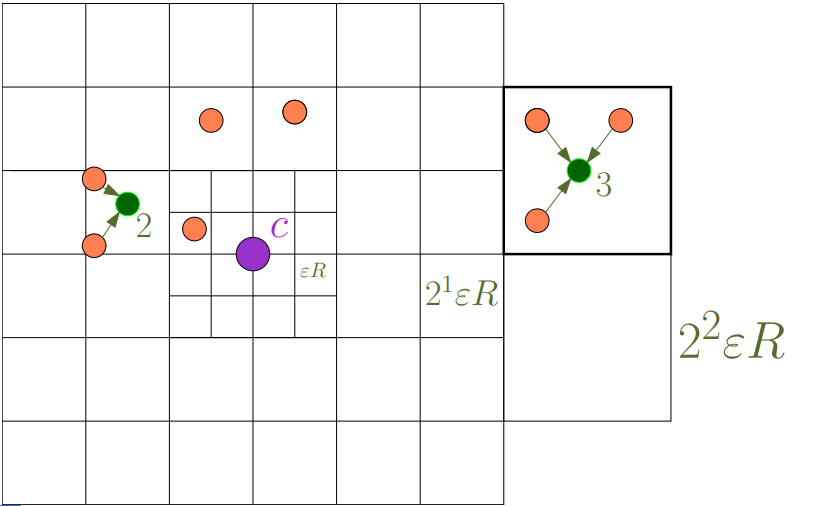
\includegraphics[totalheight=4cm]{grid.png}
    \caption{Intuicyjnie kratę wykładniczą możemy przedstawić obrazowo, gdzie $c = x_{i}$.}
\end{figure}
\noindent
Kolejnym krokiem będzie budowa kraty wykładniczej wokół każdego punktu $x_{i}$ oraz nałożenie jej na zbiór $P$.
Niech $Q_{i,j}$ będzie kwatratem o boku długości $R2^{j}$ o środku w punkcie $x_{i}$ dla $j = 0, \dots, M$, gdzie $M = \lceil 2 \lg(cn) \rceil$, który jest równoległy do osi układu współrzednych dla danej przestrzeni.
Następnie, niech $V_{i, 0} = Q_{i, 0}$ oraz niech $V_{i,j} = Q_{i,j} \setminus Q_{i,j}$ dla $j = 0, \dots, M$.
Kolejnym krokiem będzie przekształcenie $V_{i,j}$ w kratę, której komórki będą długości $r_{j} = \frac{\epsilon R2^{j}}{10cd}$ oraz niech $G_{i}$ oznacza wynikową kratę wykładniczą dla $V_{i,0}, \dots, V_{i,M}$.
Mając $G_{i}$ obliczamy dla każdego punktu z $P_{i}$, komórkę do której należy.
Dla każdej niepustej komórki z kraty wybieramy losowy punkt z $P_{i}$, który będzie jej reprezentantem.
Do takiego punktu przypisujemy wagę, która bedzie równa liczbie punktów z komórki dla której jest reprezentantem.
Po przejściu całej kraty otrzymamy zbiór $S_{i}$ takich punktów.
Definujemy $S = \bigcup_{i} S_{i}$, który jest  $(\epsilon, k)$ coresetem.
Zauważmy, że $|S| = O\Big( \frac{|A| \log n }{ (c\epsilon)^{d} } \Big)$, ponieważ każda krata ma $\log n$ poziomów, a każdy poziom stałą liczbę komórek.
\begin{proof}
    TBA
\end{proof}
